%用来打印中文
\documentclass[UTF8]{ctexart}
\RequirePackage{iftex}
\RequirePackage{fix-cm}
\RequirePackage{fixltx2e}
%页面设置
\RequirePackage{geometry}
\if@twoside
 \geometry{a4paper,
 bindingoffset = 2cm,
 inner = 0.5cm,
 outer = 2cm,
 top = 3cm,
 bottom = 2cm
 }
\else
 \geometry{a4paper,
 left = 2cm,
 right = 2cm,
 top = 2cm,
 bottom = 2cm
 }
%各种包
\usepackage{fancyhdr}
\usepackage{amssymb}
\RequirePackage{graphicx}
\RequirePackage{subfigure}
\RequirePackage{caption}
\RequirePackage{diagbox}
\RequirePackage{multirow}
\RequirePackage{makecell}
\RequirePackage{booktabs}
%\usepackage{lipsum}
\usepackage{mathtools}
\usepackage{listings}%代码
%矩阵
\usepackage{amsmath,xcolor}
\RequirePackage{longtable}
\RequirePackage{array}
%页眉
\RequirePackage{float}
\RequirePackage{flowchart}
\pagestyle{fancy}
\renewcommand{\headrulewidth}{0.5pt} 
\lhead{} \rhead{whh\ allesgutewh@gmail.com}%\thepage
% 顶格写\noindent
\begin{document}
%\pagenumbering{arabic}
\section*{Information Theory Homework-ch9}
%姓名(学号)第x章作业.pdf
\begin{center}
\today
\end{center}
\subsection*{Assignments}


9.2,\  9.3,\  9.6,\  9.7,\  9.8,\  9.9


\subsection*{9.2•双输出的高斯信道}
不妨设X均值为零。
\begin{equation*}
    \begin{split}
        C =& max I(X;Y_1,Y_2)\\
        I(X;Y_1,Y_2)=& h(Y_1,Y_2) - h(Y_1,Y_2|X)\\
        =& h(Y_1,Y_2)-h(Z_1+X,Z_2+X|X)\\
        =& h(Y_1,Y_2)-h(Z_1,Z_2|X)\\
        =& h(Y_1,Y_2)-h(Z_1,Z_2)\\
        =& h(Y_1,Y_2) - \frac{1}{2}log(2\pi e)^2|K|\\
        =& h(Y_1,Y_2) - \frac{1}{2}log(2\pi e)^2N^2(1-\rho ^2)\\
    \end{split}
\end{equation*}

$\because E(Z_1)=E(Z_2)=0$

$\therefore Var(Y_1)=E(X+Z_1)^2 = P+N,\quad Var(Y_2)=E(X+Z_2)^2 = P+N$

$\quad Cov(Y_1Y_2)=E(X+Z_1)(X+Z_2)=P+\rho N$

\[
    \therefore
    K_Y = \begin{bmatrix}
     N+P & P+\rho N \\
     P+\rho N& N+P
    \end{bmatrix}
\]

$\therefore I(X;Y_1,Y_2)=\frac{1}{2}\log \frac{|K_Y|}{N^2(1-\rho^2)}=\frac{1}{2}\log(1+\frac{2P}{N(1+\rho)})$

(a)$\rho =1\  (Z_1=Z_2)$


$ C = \frac{1}{2}log (1+\frac{P}{N})$

(b)$\rho =0$

$C \frac{1}{2}\log(1+\frac{2P}{N})$


(c)$\rho =-1\ (Z_1+Z_2 = 0)$

$ C = \infty$

\subsection*{9.3•输出功率约束}
考虑期望输出功率约束条件P的AWGN信道,即,$Y=X+Z\sim N(0,\sigma ^2)$,Z和X相互独立,并且$EY^2\leqslant P$。求其信道容量。

\begin{equation*}
    \begin{split}
        C =& max I(X;Y)\\
        I(X,Y)=& h(Y) - h(Y|X)\\
        =& h(Y) - h(X+Z|X)\\
        =& h(Y)-h(Z)\\
        =& h(Y)- \frac{1}{2}\log 2\pi e N
    \end{split}
\end{equation*}

$\because EY^2\leqslant P$

$\therefore h(Y)\leqslant \frac{1}{2}\log 2\pi e P$

$\therefore C = max I(X;Y)= \frac{1}{2}\log \frac{P}{N}$, 当且仅当$EY^2= P$且Y符合高斯分布时取等号。
\subsection*{9.6•并联信道与注水法}
由注水法,临界条件为$\sigma_1^2-\sigma_2^2=2P$

\begin{figure}[h]
    \centerline{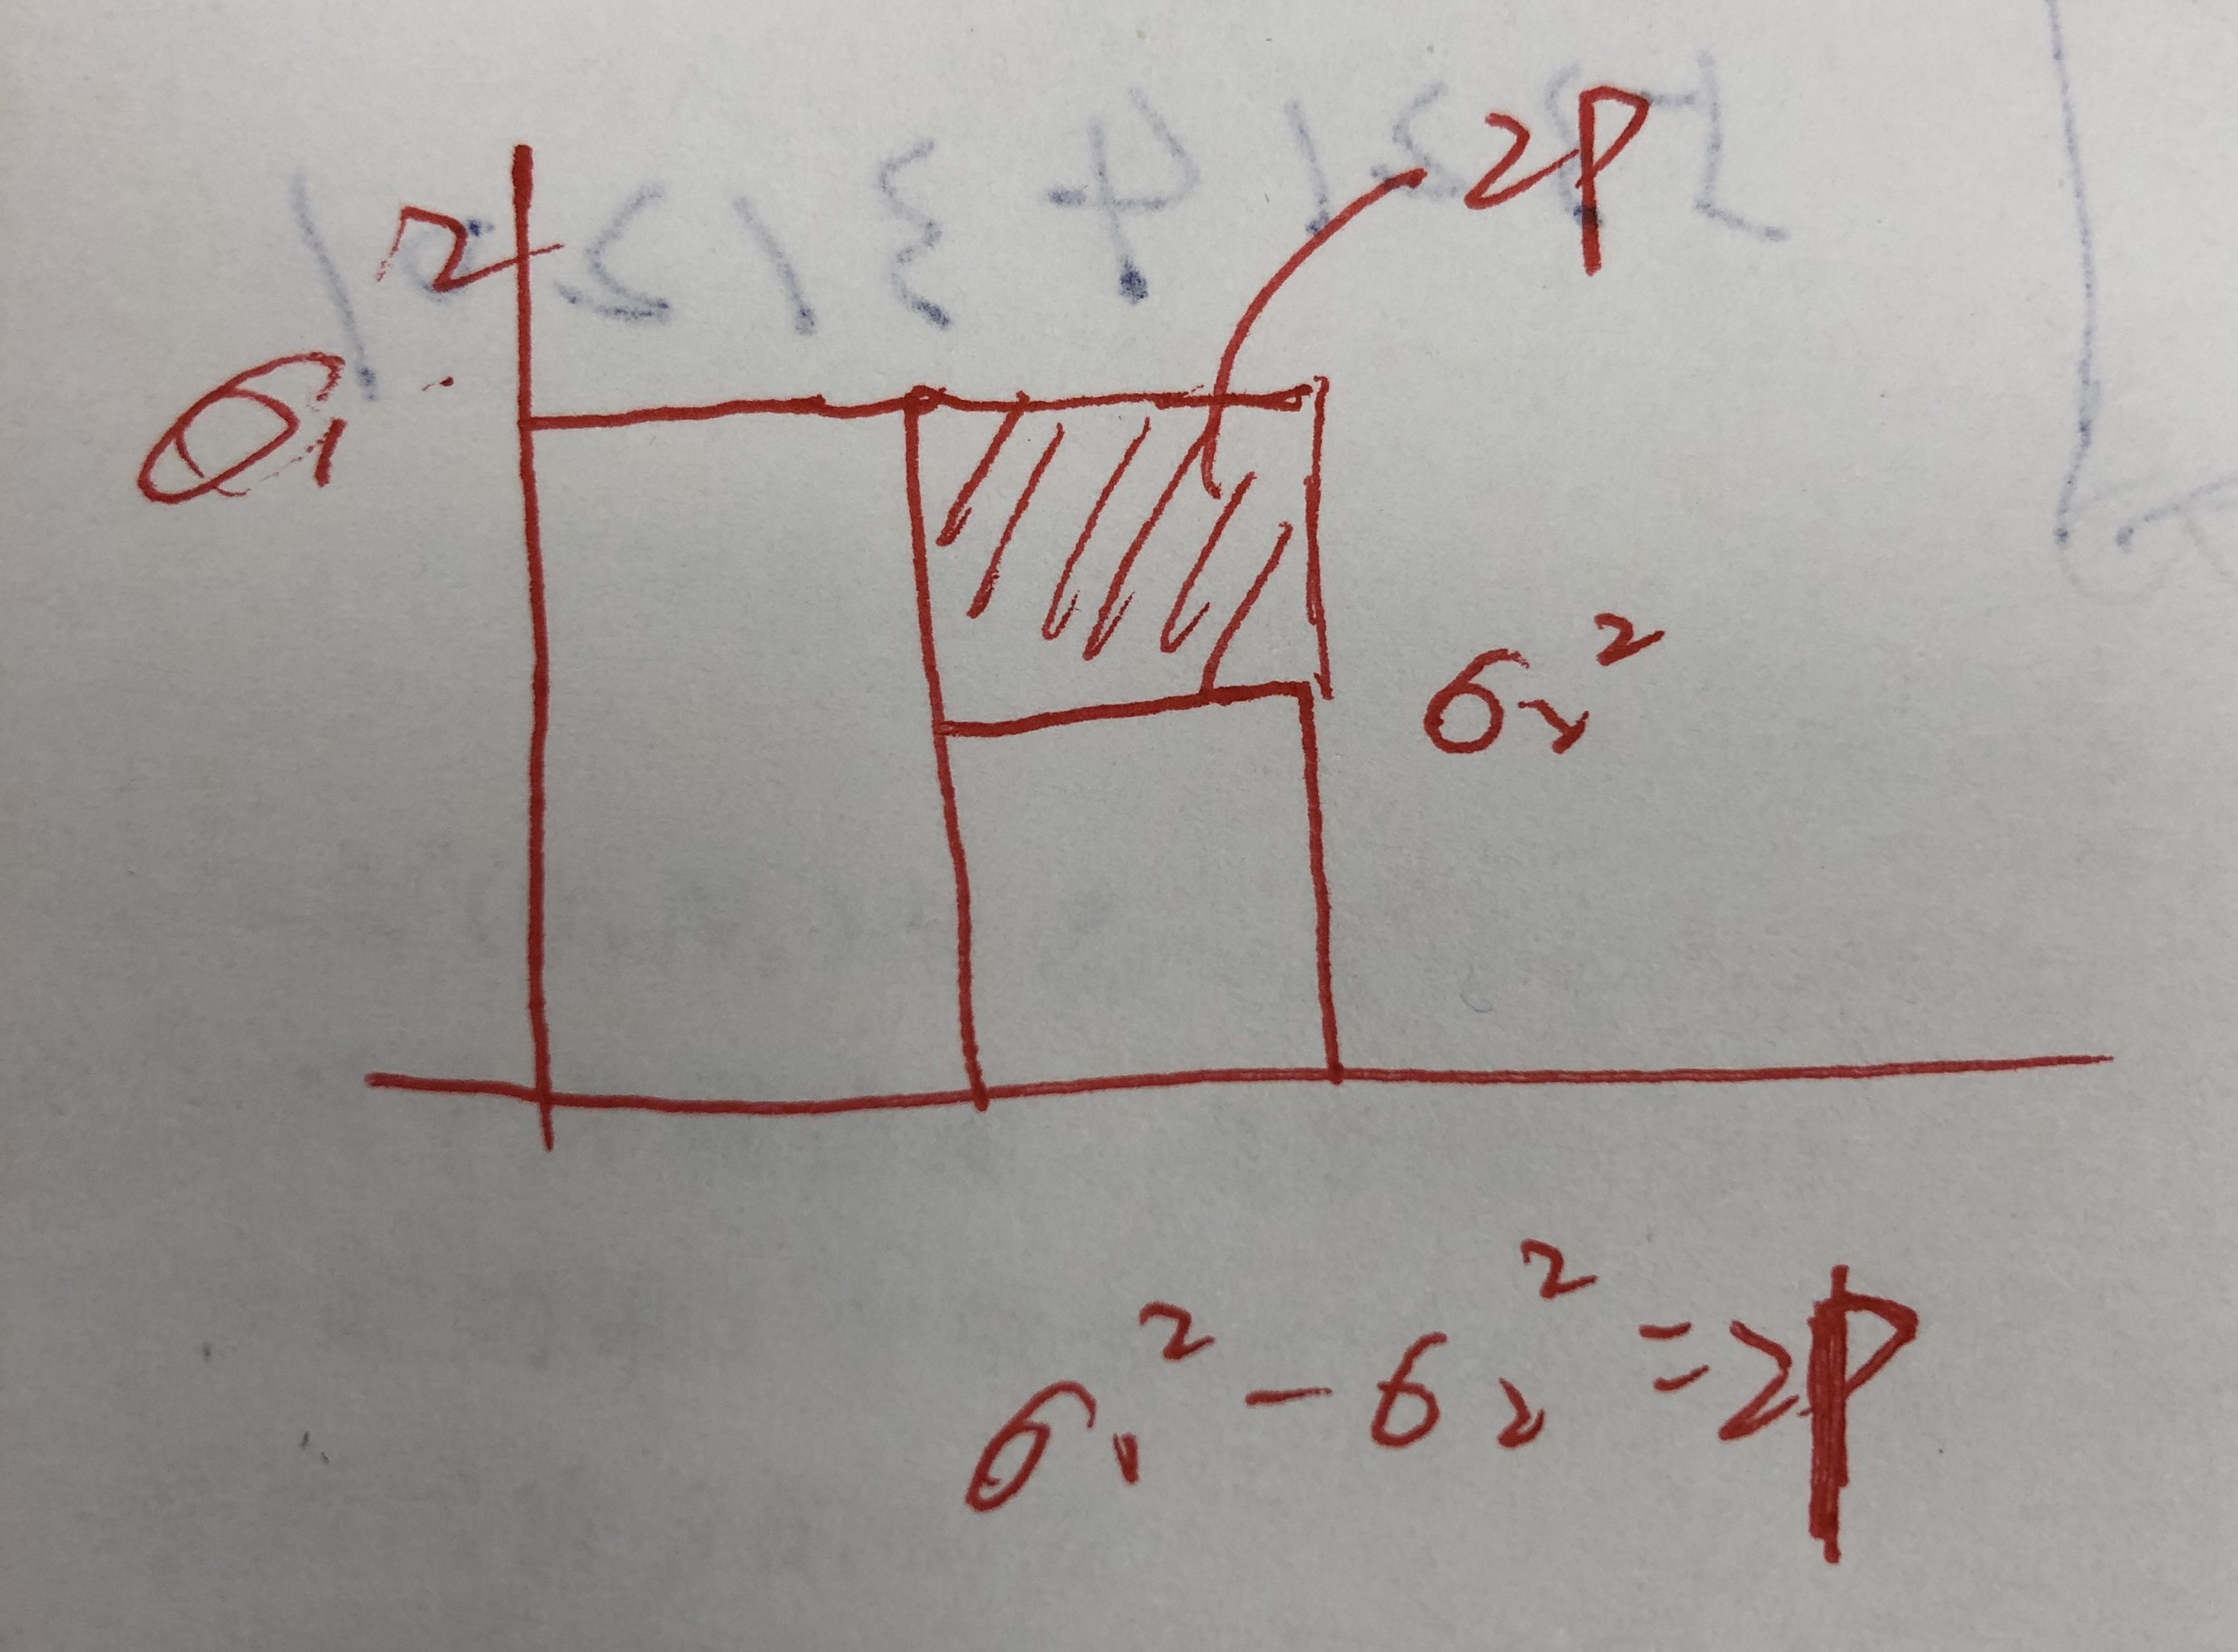
\includegraphics[totalheight = 1.5in]{ch9-6.jpg}}
    \caption{9.6示意图}
    \end{figure}
\subsection*{9.7•多路高斯信道}
(a)\begin{equation*}
    \begin{split}
        C =& max I(X;Y)\\
        I(X,Y)=& h(Y) - h(Y|X)\\
        =& h(2X+Z_1+Z_2) - h(2X+Z_1+Z_2|X)\\
        =& h(2X+Z_1+Z_2)-h(Z_1+Z_2)\\
    \end{split}
\end{equation*}

不妨设X,$Z_1$,$Z_2$期望均为0。

$ Var(Z_1+Z_2)=E(Z_1+Z_2)^2=\sigma^2+2\rho\sigma^2+\sigma^2 = 2\sigma^2(1+\rho)$

$Var(2X+Z_1+Z_2)=E(2X+Z_1+Z_2)^2=4P + 2\sigma^2(1+\rho)$

$\therefore C = max I(X;Y)=\frac{1}{2}log (1+ \frac{2P}{\sigma^2(1+\rho)})$

(b)

$\rho = 1, C =\frac{1}{2}log (1+ \frac{P}{\sigma^2})$

$\rho = 0, C =\frac{1}{2}log (1+ \frac{2P}{\sigma^2})$

$\rho = -1, C =\infty$

\subsection*{9.8•并联高斯信道}
KKT:
\begin{equation*}
    \begin{split}
        &L = \sum_{i = 1,2}\frac{1}{2}\log (1+\frac{P_i}{N_i})+\lambda (\sum_{i=1,2}\beta_iP_i-\beta)-\sum_{i=1,2}\pi_iP_i\\
        &\frac{\partial L}{\partial P_i}=-\frac{1}{2(P_i+N_i)}-\pi_i=0\\
        &\lambda (\beta_1P_1+\beta_2P_2-\beta)=0\\
        &\pi_iP_i=0
    \end{split}
\end{equation*}

$\lambda = 0$时,$P_i=-\frac{1}{2\pi_i}-N_i<0$,显然不成立,故有$\lambda \neq 0, \sum_{i=1,2}\beta_iP_i=\beta$;

$P_i\neq 0$时,$\pi_i = 0\Rightarrow P_i=\frac{1}{2\lambda\beta}-N_i$;

$P_i= 0$时,$\pi_i \neq 0\Rightarrow \frac{1}{2\lambda\beta}-N_i<0$;

$\therefore \sum_{i=1,2}(\frac{1}{2\lambda\beta_i}-N_i)^+=\beta,\ P_i = (\frac{1}{2\lambda\beta_i}-N_i)^+,\ \beta_iP_i=(\lambda^\prime - N_i\beta_i)^+\ (\lambda ^\prime = \frac{1}{2\lambda})$

(a)由题意知,$N_i, \beta_i$为固定值,

$N_1\beta_1\geqslant N_2\beta_2 $时临界条件为$(N_1\beta_1 - N_2\beta_2) = \beta$;

$N_1\beta_1< N_2\beta_2 $时临界条件为$(N_2\beta_2 - N_1\beta_1) = \beta$;


(b)由题意$10 = (k-3)^++(k-4)^+$,带入(a)计算得到超过临界值,此时表现为双信道,则$10 = (k-3)+(k-4)\Rightarrow k=\frac{17}{2}\Rightarrow  P_1=\frac{11}{2}, P_2 = \frac{9}{4}$
\subsection*{9.9•向量高斯信道}
不妨设X均值为零。

\begin{equation*}
    \begin{split}
        C =& max I(X;Y)\\
        I(X;Y)=&h(Y)-h(Y|X)\\
        =& h(X+Z)-h(Z)\\
    \end{split}
\end{equation*}

$r(K_Z)=2<3\Rightarrow |K_Z|=0\Rightarrow h(Z)=-\infty\Rightarrow C=\infty$

\end{document}
